\section{Line Plot \cite{wiki-line-chart}}\label{plot_line}
A line chart or line graph, also known as curve chart, is a type of chart that displays information as a series of data points called 'markers' connected by straight line segments. It is a basic type of chart common in many fields. It is similar to a scatter plot except that the measurement points are ordered (typically by their x-axis value) and joined with straight line segments. 


\begin{table}[H]
    \begin{minipage}{0.45\textwidth}
        \centering
        \begin{tabular}{|c|c|}
            \hline
            Elapsed Time ($s$) & Speed ($m/s$) \\ \hline
            0 & 0 \\ \hline
            1 & 3 \\ \hline
            2 & 7 \\ \hline
            3 & 12 \\ \hline
            4 & 18 \\ \hline
            5 & 30 \\ \hline
            6 & 45.6 \\ \hline
        \end{tabular}
        \caption{Data: Line Plot}
    \end{minipage}
    \hfill
    \begin{minipage}{0.45\textwidth}
        \begin{figure}[H]
            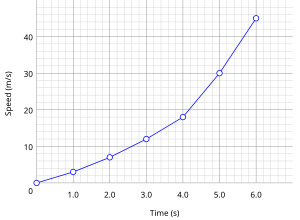
\includegraphics[width=\linewidth]{Pictures/data/data_line_chart.jpg}
            \caption{Graph: Line Plot}
        \end{figure}
    \end{minipage}
\end{table}
